\documentclass[]{Photos_interface_design}
\usepackage{graphicx}
\usepackage{hyperref}
\usepackage{eurosym}
\usepackage{pifont}
%\usepackage{tocloft}
\usepackage{amsmath}
\usepackage{subfigure}
\usepackage{booktabs}

\makeatletter
\renewcommand*\l@subsection{\@dottedtocline{2}{1.5em}{2.0em}}
\renewcommand*\l@subsubsection{\@dottedtocline{3}{3.0em}{3.0em}}
\makeatother

\begin{document}

\maketitle

\tableofcontents\pdfbookmark[0]{Table of Contents}{toc}

\newpage

\section{Introduction}
For a long time, {\tt PHOTOS} Monte Carlo \cite{Barberio:1990ms,Barberio:1993qi} has been used for the generation of bremmstrahlung in the decay of particles and resonances. Over the years the program has acquired
popularity and discussion of its systematic error have pushed it to high 
precision \cite{Golonka:2006tw}. Multiphoton radiation was introduced \cite{Golonka:2005pn}, phase space treatment was shown to be exact \cite{Nanava:2006vv} and for several processes \cite{Golonka:2006tw,Nanava:2006vv,Nanava:2009vg}
an exact matrix element was introduced with the help of optional weights.
Benchmarks distributions, including comparisons with  
other simulation programs, were collected on the program web page \cite{Photos_tests}. 

 Such high precision applications require good control of the event record content on which {\tt PHOTOS} operates. On one side it 
requests skills and experience of the user and on the other it provides 
the flexibility necessary for the study of effects like systematic errors for 
measurements of anomalous couplings or W mass for example. Methods of 
correlated samples  can be applied\footnote{To exploit such methods in 
the high precision regime, good control of matrix element properties is necessary
\cite{Kleiss:1990jv}} 

Until recently {\tt HEPEVT} was used as the structure for 
communication between physics Monte Carlo programs and detector/reconstruction 
packages. Experimental physicists used HEPEVT 
for their own applications  as well.

Recently, to gain  flexibility, {\tt FORTRAN} is begin replaced by C++ and 
instead of {\tt HEPEVT}, the C++ event structure called {\tt HepMC} \cite{Dobbs:2001ck}
is used. Nothing prevents 
moving {\tt PHOTOS} to an environment based on  {\tt HepMC}
and to rewrite the whole (begining with the event record interface)
of {\tt PHOTOS}\footnote{An up-to-date version of the code described in this paper is
available from the web page of our project~\cite{photosC++}. 
As we are still in the phase of refining
we change the program (and update this note) on a regular basis. 
This can be a problem if bug fixing is necessary and the user has invested time 
in a temporary version. To overcome this difficulty, 
together with the code, information of the code version in 
SVN is available.  }

 to C++. In fact implementation of the algorithm is clearer and easier to
 maintain. Because of its design the {\tt PHOTOS} algorithm benefit from the object 
oriented features of C++. It is our third program, after {\tt MC-TESTER} \cite{Davidson:2008ma}
and the {\tt TAUOLA} interface \cite{Davidson:2010rw} previously ported to {\tt HepMC} and C++.
This completes the main step of migration of these 3 programs to the new style.

Such migration is convenient for the users too,  they can now work
with  homogenous C++ software. From the physics point of view transformation 
of {\tt PHOTOS} 
from {\tt FORTRAN} to C++  brings some benefits as well.
The channel dependent, complete first order matrix elements of {\tt PHOTOS}, in {\tt FORTRAN},
 are available only 
in special
kinematical configurations. With the help of new event record interface they will become
available for general use.
For that purpose, better access to information necessary to orient spin state of the decaying particles
will be provided already now.



Our paper is organized as follows ...\textbf{nd-text is missing here}



\section{Requirements of the {\tt PHOTOS} Interface}
The algorithm of {\tt PHOTOS} Monte Carlo can be divided into two parts.
An internal one, operates on elementary decays. Thanks to carefully 
studied properties of the 
QED (scalar QED) algorithm, with certain probability, 
replace  kinematical configuration of Born level decay by a new one, 
where bremsstrahlung photon or photons
are addeed and other particle momenta modified. This part of the program is sophisticated from the physics 
point of view \cite{Nanava:2006vv,Golonka:2006tw},
but from the point of view of data structures the algorithm is simple.
That is why, the gain from re-writing this part of the program to C++ is rather
limited and will be postponed to a later step of the project development.
On the other hand, there are not many obstacles for such a transformation to be
performed. In fact such a transformation was performed already
previously \cite{photosplus}, but the resulting program was developed too early 
and did not attracted users.

The typical result of high energy process simulation are events of complex structure
they include for example initial state parton showers, hard scattering parts,
hadronization and finally chains of cascade decays of resonances. 
A structure similar to a tree is created, but properties of such tree type data structures
are sometimes violated.
For its action {\tt PHOTOS} needs to scan an event record (tree) 
and localize branchings where
it is supposed to act. The decaying particle (mother) and its primary decay products
(daughters) have to be passed into the internal event structure of {\tt PHOTOS}. 
Finally for each daughter a list of all its subsequent decay products has to be 
formed. It is needed as kinematical modifications need to be performed on each 
member of the list according to the change introduced to the primary daughter.

In the new C++ version of this part of the algorithm additional functionality
is provided.
First mother of the decaying particle will be localized and passed together with  
elementary branching to internal part of the program. 

Prior to activation
of the {\tt FORTRAN} part of the algorithm all decay branching 
(supplemented with the first 
mother) will be boosted to decaying particle rest frame and first mother
will be oriented along z axis.
mother) will be boosted into the decaying particle's rest frame and the first mother
will be oriented along the z axis.
%\textbf{nd-it might be worth defining what the FORTRAN part of the algorithm is. Although you explain in the introduction, people might not link the two. ZW: but we write Prior to activation of the {\tt FORTRAN} part}.

We can summarize that the following operations must be implemented
in our event record interface:
\begin{enumerate}
\item a method to search for elementary decays over entire tree of the event.
\item a method to form lists of all subsequent decay products originating from each elementary decay product.
\item a method to localize the first mother of a decaying particle. 
\item a method to localize the  second mother of a $t \bar t$ pair.
\item a method to read  particles stored in the event tree.
\item a method to add or modify particles of the event tree.
\end{enumerate}

TXT\footnote{ {\bf remnant text to be removed. Parts may be moved to other places.}  

{\tt PHOTOS} act on such vertex and modifies four momenta of residing there daughters 
and eventually adds new ones that is photons. 
Such procedure is exact from the point of view of phase space; for details see eg.  approximation in on flight constructed matrix elements are based
on factorization properties of QED. 

In case one is interested to go beyond that precision level, one has to  provide
more information. Spin state of the decaying particle has to be passed to the code calculating matrix element. For that it is enough to store into event record
information on particles or fields resulting in creation of
our particle under consideration that is mother for the decay vertex.
It is then convenient to transform all particles to the rest frame of the Mother
and orient Mothers mother along z axis before passing the information from HepMC to {\tt PHOTOS} internal data structure. Let us call resulting Lorentz transformation $L$. Once PHOTOS internal algorithm complete
its action all four momenta have to be transformed back by $L^{-1}$ and 
modification of remaining part of the event record (replacement of momenta
add of new photons to HepMC and modification of all descendants of 
daughters would be performed as in more standard case explained above.
}

\subsection{C++ and HepMC Specific Requirements}

The C++ version of the {\tt PHOTOS} interface implements all functionalities
of its predecessor, the {\tt PHOTOS} coded in {\tt FORTRAN}.
It can be attached to any Monte-Carlo program,
provided its output is available through a {\tt HepMC} \cite{Dobbs:2001ck} event record.

This condition is not very restrictive, is seems that {\tt HepMC} will
remain a generally accepted standard for the near future. However,
already now several different options for how {\tt HepMC} is used are
widespread. Possibility of the flexible  adaptation of our event record 
interface to different
options has been considered in the design,  drawing experience
from {\tt MC-TESTER} \cite{Golonka:2002rz,Davidson:2008ma}.
We have also
envisaged the possibility that {\tt HepMC} may one day be replaced by another
standard of event record, and we have provided an easy way to extend
the interface to a possible new event record standard.

\subsection{Object Oriented Event Records  -- The Case of {\tt HepMC}}
\textbf{nd-the next paragraph repeats information
  that's already stated in other places. will }
 In adopting the {\tt PHOTOS} interface to the C++ event record format
the difference between the {\tt HEPEVT} event record used in the {\tt
  FORTRAN} version of the {\tt PHOTOS} interface and {\tt HepMC} event
record which is used for the C++ based interface has to be taken into
account.  In the first case 
common block containing a list of particles with their properties and
with integer variables denoting pointers to their origins and
descendants is used.  The {\tt HepMC} event structure is built from vertices,
each of them having pointers to their origins and descendants. Links
between vertices represent particles or fields.  Fortunatelly in both, {\tt
  FORTRAN} and C++ cases, the event is structured as a
tree\footnote{At least in principle, because in practice its
properties may be rather of a graph without universally defined
properties.  This makes our task challenging.}, the necessary
algorithms are analogous, but nonetheless different. The {\tt HepMC}
structure based on vertices is more convenient for the {\tt PHOTOS}
interface. 

In {\tt HepMC version 2.04}, an  event is represented by a {\tt GenEvent} object,
which contains all information regarding itself, including event id,
units used for dimensional quantities in the event and the list of produced particles. The particles
themselves are grouped into {\tt GenVertex} objects allowing access to mother
and daughter particles of a single decay. Vertices provide an easy way
to point to the whole branch in a decay tree that needs to be accessed,
modified or deleted if needed. The information of a particle  itself is stored
in a {\tt GenParticle} object containing the particle id, status and momentum
as well as information needed to locate its position in the decay tree.
This approach allows traversing the event record structure in several different
ways.

The {\tt HepMC} event record format is  evolving with time, making it necessary
 to adapt
the code to the new versions.
{\tt HepMC} version 2.05 is used as a default for our distribution and tests. 
In the case of version 2.03 restrictions on methods for 
units
conversion have to be taken into account, for details see Appendix B.5
of ref. \cite{Davidson:2010rw}. At present we have not yet introduced such 
backward compatibility downgrade for {\tt PHOTOS}. It is probably not necessary.
However,
one should keep in mind that future adaptations to {\tt HepMC} changes may restrain
backward compatibility.

Evolution of the {\tt HepMC} format itself is not a crucial problem.
In contrast, conventions on how physics information is  filled into {\tt HepMC}
represent the main source of technical and also physics 
challenges for our interface. 
This is quite similar to the previous
{\tt HEPEVT - FORTRAN} case. Let us discuss this point in more detail now.

\subsubsection{Event Record Structure Scenarios}

{\bf PYTHIA,HERWIG,MC@NLO etc. }

While many Monte-Carlo generators (eg.. {\tt PYTHIA 8.1} \cite{Sjostrand:2007gs}, 
HERWIG++ \cite{Bahr:2008pv})
store events in {\tt HepMC} format, the  representations of
these events are not subject to strict standards,  which can therefore
vary between Monte-Carlo generators or even physics processes. Some examples
of these variations include the conventions of status codes, the  way
documentary information on the event is added, the direction of pointers at a vertex
and the conservation (or lack of conservation) of energy-momentum at a vertex.
Below is a list of properties for basic scenario we have observed in Monte-Carlo
generators used for testing the code.

This list will serve as a declaration for convention of  {\tt HepMC} filling, which  the 
interface should  be able to interpret correctly.

\begin{itemize}
  \item \textbf{4-momentum conservation} is assumed for all vertices in the event record where {\tt PHOTOS} is expected to act.
  \item \textbf{Status codes:} only information whether given particle is incoming, outgoing or intermediate will be used. We assume the codes used will be 0,1 or 2 like in HEPEVT. All other codes will be treated as
equivalent to  the status 2.
  \item \textbf{Pointers at a vertex} are assumed to be bi-directional. That is, it is possible to traverse the record structure from mother to daughter and from daughter to mother along the same path.
\end{itemize}

\noindent
\textbf{ Extensions/Exceptions} to this specifications  are handled in some cases. We will call them
options for conventions of event record filling.
  \begin{itemize} 
    \item  Vertices like $\tau^\pm \rightarrow \tau^\pm$ and $\tau^\mp \rightarrow \tau^\mp \gamma$ 
           where 4-momentum conservation is not preserved. Due to 4-momentum non-conservation,
           {\tt PHOTOS} will not be invoked.
    \item
           As in the {\tt FORTRAN} cases, we expect that  new  types of 
           conventions for filling the event record
           will appear, because of physics motivated requirements.
           Unfortunately, the resulting options do not always guarantee
           an algebraically closed structure.  
           Host program specific patches  may need to be defined for the 
           {\tt TAUOLA interface}. 
           Debugging it could be time consuming, and would need to be repeated for every new
           case.
   \end{itemize}


Detailed
conventions for the actual filling of physics information into {\tt HepMC} format
is defined by the authors of each Monte Carlo program.
 In the future,  an important special case of event records filling with
information extracted from experimentally observed event (eg. $Z\to \mu^+\mu^-$
 modified later to $Z\to \tau^+\tau^-$) should be allowed.
  Obviously, a new type (or types) of {\tt HepMC} filling will then appear.

A good example is the evolution of {\tt PYTHIA}. While in version 8.108 status codes for 
our example processes were  taking values 0, 1, or 2  only (in the part of the record 
important for {\tt PHOTOS}), other values were already present in
version 8.135. As a consequence status code for 
otherwise nicely decaying particles were not anymore 2 only. We have introduced 
a change  in the file PhotosEvent.cxx to adjust. After  the change
program should work for all previous cases as before, however this is difficult to validate.
Further tests are necessary. We should also investigate 
if instead of changes on the side of  {\tt PHOTOS} adjustment in input of {\tt PYTHIA} would not 
be more appropriate 
solution for us and at this moment.

We need to decide on bar code conventions. Our programs, {\tt TAUOLA} and
 {\tt PHOTOS} supplement the event record with new particle entries carrying bar codes 
increased by 10000 with respect to the value which would be given if such 
particles were generated by the main generator program. 
That is the choice resulting from our use 
of {\tt HepMC} methods and defaults.  It is not clear to us if it is 
reasonable choice from the point of view of program users.

\subsection{Interface to event record of {\tt FORTRAN}}
\label{sect:F77fill}

In principle it would be rather simple to re-write the whole of {\tt PHOTOS} into
C++. However to profit from numerical tests, for the time being the numerical core of PHOTOS
is still left in {\tt FORTRAN}. The C++ part of the code searches the whole event for
suitable HepMC vertices for the generation of bremsstrahlung. Once such
a vertex is found it is copied to an internal event record  which is 
called  {\tt PH$\_$HEPEVT} (this is effectively the same structure as {\tt HEPEVT};
the event record of {\tt FORTRAN}).
The {\tt FORTRAN} code of {\tt PHOTOS} is then executed.
The data structure passed in this way is rather simple. A single vertex
supplemented with mothers of decaying particle are passed only. Information 
on mothers will be useful in future for the calculation of process dependent 
kernels. Another data structure of   {\tt HEPEVT} type, {\tt PHOEVT}, is also 
used in {\tt PHOTOS}. It is used to store the decay vertex only.  
The two structures are only temporary.


For details on the interface to {\tt FORTRAN} see appendix \ref{Interface to PHOTOS}.


\section{Design}

\subsection{Classes and Responsibilities}

The choice of splitting the source code into three main modules
 allows the separation of the {\tt FORTRAN} related code from the abstract C++ interface
and the concrete implementation of the interface created for the appropriate
event record.

\begin{figure}[h!]
\centering
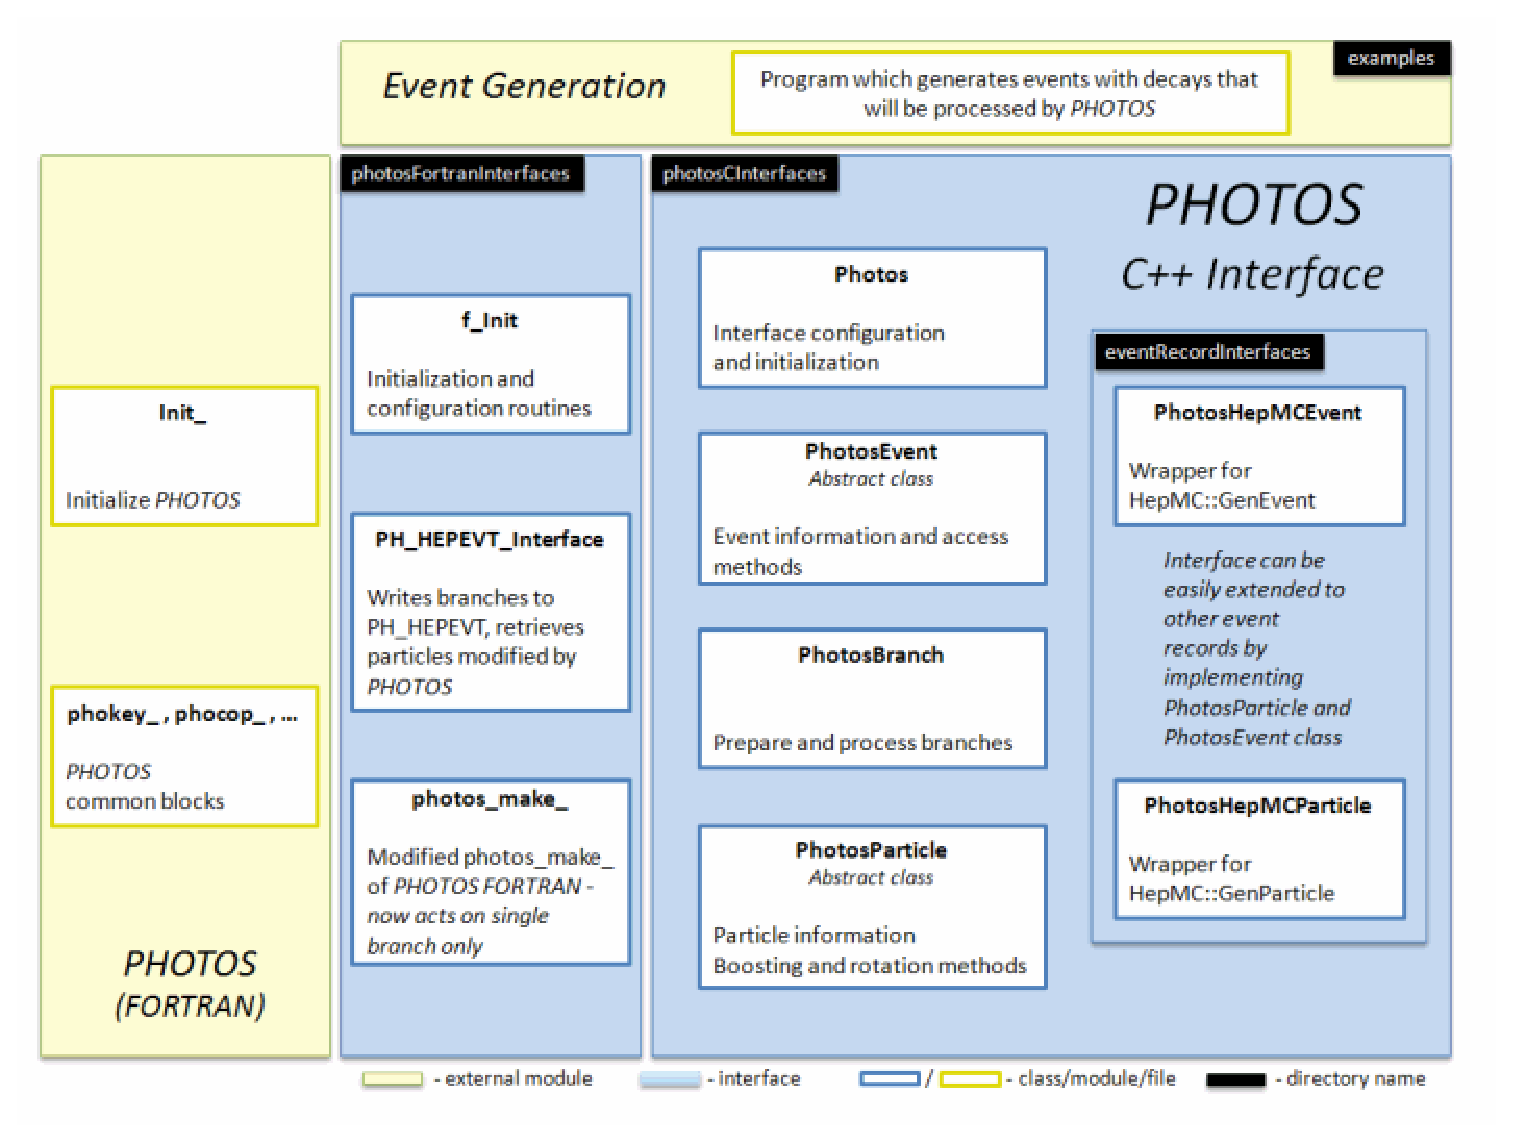
\includegraphics[scale=0.6]{interface_design.eps}
\label{fig:design}
\caption{{\tt PHOTOS} C++ interface class relation diagram}
\end{figure}

\begin{itemize}
  \item {\bf {\tt PHOTOS FORTRAN} Interface}\\
       This part of the code provides an interface 
       to the {\tt FORTRAN} library of {\tt PHOTOS}. In particular,  routines
       necessary for library initialization and a wrapper for the routine which invokes the processing
	   of a single branch. Parts of the interface code are still left in {\tt FORTRAN}, but
	   can be rather easily rewritten to C++. 
       The most important part of this module, {\tt PH\_HEPEVT\_Interface\_},
       is already implemented  in C++. This method is responsible for writing
	  the decay branch to be processed into the internal event record {\tt PH\_HEPEVT}.
       For further details see Appendix \ref{Interface to PHOTOS}.
  \item {\bf {\tt PHOTOS} C++ Interface} \\
       This is an abstract interface to the event record.
       The class {\tt PhotosEvent} contains information regarding the whole event
       structure, while {\tt PhotosParticle} stores all information regarding a single particle.
       All particles used by the interface are located in the event in the form of
       a list of {\tt PhotosParticle} objects.
       The last class located here, {\tt PhotosBranch}, contains information regarding
	 a  single branch to be processed by {\tt PHOTOS}.
  \item {\bf Event Record Interface} \\
       This contains the event record implementation classes. All classes stored here represent
       the implementation of specific event record interfaces and are responsible for reading,
       traversing and writing to the event record structure.
       Only the {\tt PhotosEvent} and {\tt PhotosParticle} classes must be implemented.
       The {\tt HepMC} event record interface is implemented
       through {\tt PhotosHepMCEvent} and {\tt PhotosHepMCParticle}. These classes are similar to the
       analogous TAUOLA event record classes.
\end{itemize}

\subsection{Directory Structure}

\begin{itemize}
\item {\bf src/eventRecordInterfaces/ } - source code for classes which interface with {\tt HepMC}.\\
  Classes:
  \begin{itemize}
  \item { \bf PhotosHepMCEvent} - interface to HepMC::GenEvent objects. 
  \item { \bf PhotosHepMCParticle} - interface to HepMC::GenParticle objects. 
  \end{itemize}   

\item {\bf src/photosCInterfaces/ } - source code for general {\tt PHOTOS} interface.  \\
  Classes:
  \begin{itemize}
  \item { \bf Photos } - controls the configuration and initialization of {\tt PHOTOS FORTRAN}.
  \item { \bf PhotosEvent } - abstract base class for event information.
  \item { \bf PhotosParticle } - abstract base class for particles in the event.
  \item { \bf PhotosBranch } - contains one {\tt PhotosParticle}, and  pointers to its mothers and daughters.
  Filtering branches sent to {\tt PHOTOS} is done here.
  \end{itemize}

\item {\bf src/photosFortranInterfaces/ } -  interface to {\tt PHOTOS FORTRAN} routines and common blocks. \\
  Files:
    \begin{itemize}
    \item { \bf f\_Init } - contains a wrapper for the {\tt PHOTOS FORTRAN} routines for initialization.
    \item { \bf PH\_HEPEVT\_interface } - contains a wrapper for accessing PH\_HEPEVT common block.
    \item { \bf photos\_make.f } - contains extra {\tt FORTRAN} routines which should ultimately be migrated to C++.
    \end{itemize}

\item {\bf src/utilities/ } - source code for utilities that help with debugging.\\
  Classes:
  \begin{itemize}
  \item { \bf Log} - general purpose logging class that allows filtering out output messages 
      of {\tt PHOTOS C++ Interface} and tracks statistics for each run.
  \end{itemize}   

  \item {\bf examples/ } - examples of different {\tt PHOTOS} C++ Interface uses.
    \begin{itemize}
	\item {\bf photos\_standalone\_example} - the most basic example which loads pre-generated 
	      events stored in a file in {\tt HepMC} format which are then processed by {\tt PHOTOS}.
	\item {\bf single\_photos\_gun\_example} - an example of using the {\tt processOne} method
	      to process only selected particles within the event record.
    \item {\bf photos\_pythia\_example} - a simple $e^+e^- \rightarrow Z \rightarrow e^+e^-$ event in
	{\tt HepMC} format which is then processed by {\tt PHOTOS}.
    \item {\bf tauola\_photos\_pythia\_example } - an example of  {\tt TAUOLA} linked with {\tt PYTHIA 8.1},
	the decay chain processed by {\tt PHOTOS} and analysed with  {\tt MC-TESTER}.
    \end{itemize}   
  \item {\bf include/} - directory for the header files.
  \item {\bf lib/ } - directory for the compiled  libraries. 
  \item {\bf documentation/ } - contains doxygen documentation and this latex file.
  \item {\bf photos-fortran/ } - the  standard {\tt PHOTOS FORTRAN} distribution
\end{itemize}

\subsection{Algorithm Outline}
\label{sect:Outline}

An overview of the algorithm for  the {\tt PHOTOS C++ Interface} is
given below. For clarity, the example assumes that the processed event
is stored in the {\tt HepMC} event record structure.

The first step is creation of a {\tt PhotosHepMCEvent} object from
a {\tt HepMC::GenEvent} event record. After that, the {\tt process()} method should
be executed by the user's code\footnote{Prior to this step
the user may want to execute {\tt Photos::processParticle(...)} or {\tt Photos::processBranch(...)}
for branches, where {\tt PHOTOS} is expected not to work properly or if only one branch
needs to be examined by {\tt PHOTOS}. For details see Appendix~\ref{PHOTOSgun}.
}, invoking the following process:

\begin{enumerate}
\item The {\tt HepMC} event record is traversed and a list of all decaying
      particles is created.
\item Each particle is checked and if it's a self-decay\footnote{History entry in event record, like
      $Z\to Z$ or $\tau \to \tau$}, the particle is filtered out.
\item For each remaining particle a branch containing the particle's mothers and daughters
      is created. Special cases mothers and daughters but no intermediate particle are handled and the
	  list of branches is created.
\item Branches are filtered out depending on the user's choice of processes
      to be skipped by {\tt PHOTOS}.
\item Each branch is processed by {\tt PHOTOS} separately:

	\begin{enumerate}
  
	\item The branch is written to PH\_HEPEVT
	\item {\tt PHOTOS} is invoked with the index of the particle from which the branch
	      has been created
 	\item The resulting branch is taken back from PH\_HEPEVT and any changes made by {\tt PHOTOS} are 
           integrated into the event record. New particles are created and the old ones are modified
		  accordingly.

	\end{enumerate}

\end{enumerate}

The underlying HepMC::GenEvent is hence modified with the  insertion of photons.

\section{Extensibility}

 The purpose of the present version of the C++ interface to {\tt PHOTOS} is to enable 
all the functionality of its {\tt FORTRAN} predecessor to be available for the HepMC data
structure. Some methods for improved initialization are already introduced in this version. New program 
functionality has been prepared to enable further extensions in the future. 
Let us briefly discuss some of these points.

\subsection{{\tt PHOTOS} Extensions}
In this paper we have presented an algorithm as it is today. 
That is, a version which is compatible with the one implemented in {\tt FORTRAN}.

\begin{itemize}
\item
As can be seen from the text presented, we have prepared the structure 
for the implementation of channel dependent matrix elements. This work, scattered
 over special corrections to the {\tt FORTRAN} version applicable one at a time can  
be simply integrated all together into C++ version. This is not urgent.
 We are  not convinced if such complication is worth 
the complication for the user as it requests more strict control of the event 
record content. Gain of precision is 
not that important because the precision is quite good already now. 
This is why we have not completed the migration of these aspects to C++.
Instead, as an intermediate step, we developed validation techniques
for the program. These are required prior to a re-write of the
numerically sensitive part of the program (which is algorithm-wise
rather simple).

\item
Methods deviced to check the content of HepMC as used by {\tt PHOTOS} were already 
described in Appendix \ref{App:Logging}. 
They need to be used whenever {\tt PHOTOS} 
processes events from a new generator eg. upgraded versions of  {\tt PYTHIA},
which may fill the event record is unexpected ways.
Experince over many years of developing and maintaining the algorithm
have shown that this is the most demanding task; the necessity to
adapt to varying physics and technical input of the event record pose
a multitude of problems. The nature of these difficulties can not be
predicted in advance. 

\item
For the sake of debugging we have introduced control methods which activate
internal printouts of the {\tt FORTRAN} part of the code.
The routine PHLUPA \cite{Barberio:1993qi} can be activated  to verify 
how an event is constructed/modified, and to investigate energy 
momentum conservation or other inconsistencies.
This is quite convenient for tracing inconsistencies in the
information passed to {\tt PHOTOS} for example.


\item
Numerical stability is another consideration; it can not be separated from
physics constraints. The condition  $E^2-p^2=m^2$ may be broken  because of 
rounding errors.  However, due to intermediate particles with
  substantial widths, this on mass shell condition may not be applicable.
{\tt PHOTOS} may be adapted to such varying conditions, but it requires
good interaction with users. Protection reversing some 
inconsistencies in the event record may be the source of unexpected difficulties
for other cases. 
At present such methods are left to the {\tt FORTRAN} part of the algorithm, 
which
will be gradually reviewed and  migrated to C++
\end{itemize}

 
\subsection{Event Record Interface}
In the times of {\tt FORTRAN}, the {\tt PHOTOS} interface used an internal event structure which was
based on HEPEVT,
adding to it (understood as a data type) an extra variable defining 
the status of particles with respect to QED Bremsstrahlung. In some cases, like
$\tau \to l \nu_l \nu_\tau$, bremsstrahlung was already generated earlier
At present, instead of such an arrangement, a set of initialization methods are 
prepared and described in section \ref{section:suppress}. 

There is definite room for 
improvement. For example if the vertex $q \bar q \to l^\pm l^\mp g$ is encountered,
the interface could `on the fly' add an intermediate $Z$ into the record and enable {\tt PHOTOS}
on the temporarily constructed decay branch $Z \to l^\pm l^\mp $. 

Internally in the {\tt FORTRAN} part of {\tt PHOTOS}, the data
structures based on HEPEVT: PH\_HEPEVT and PHOEVT, are used, but they
store a single elementary decay only. At this step in the program
evolution it might not be the most elegant solution, but it prevents
the need to redo many of the {\tt FORTRAN} era benchmarks.






\section{Testing}

One of the most important parts of the {\tt PHOTOS} project are its physics oriented tests.
Several domains
of physics tests should be mentioned. For users interested in precision 
simulations of Z or W decay the most interesting will be the papers \cite{Nanava:2009vg,Golonka:2006tw}. There, careful comparison with the first order matrix element 
and confirmation that the algorithm scheme  is compatible with exclusive 
exponentiation was the prime target. Compatibility of the solution
with a second order matrix element are less important. 
It is important to know that missing in the first order EEX or CEEX \cite{koralz4:1994,kkcpc:1999} 
scheme terms
lead to effects which are typically of the order of 0.2 \% but are at the level 
or 30 \% or more in the double hard photon region of the phase space. That is 
why it may lead to effects which are more important when complex experimental 
cuts are applied\footnote{We thank Andy Buckley for checking numerically
 that this limitation is present in many presently used monte Carlo programs,
in particular Sherpa and Herwig++.  } 
for the measurements of $W$'s or $Z$'s.
For users interested in the simulation of
background for Higgs searches at the LHC and for any other applications where 
two hard photon configurations are important, studies based on the comparison with 
double photon matrix element are of 
interest \cite{Barberio:1993qi,RichterWas:1994ep,RichterWas:1993ta}.
Finally users interested in low energy processes where the underlying physics model 
for photon emission can not be controlled in full by theory; scalar QED may 
be considered only as the starting point, will profit 
from \cite{Nanava:2009vg,Nanava:2006vv}. In all cases it is important that
the  program generation cover the full phase space and that there are no 
approximation in phase-space. As in {\tt FORTRAN} version the code 
features approximation in the kernel. In some cases the process dependent 
complete first order 
kernel is available but is not installed in the public version  
because the resulting approximation is 
numerically unimportant and requires control of the spin state for the decaying 
particle. This requires better control of the event record than what was available 
in {\tt FORTRAN}. At present such an option is prepared, see section \ref{sect:F77fill} but not exploited. 

The main purpose of the present paper is program documentation. This is why
we concentrate on the program tests required to guarrantee its proper installation.
The physics tests discussed above 
do not guarrantee that the program will perform well on a particular platform and installation. Tests and debugging
is necessary.  If the content of the event record is non-standard or rounding errors are large, the performance of {\tt PHOTOS} will deteriorate.


The first check after installation of {\tt PHOTOS} is whether some energy momentum non 
conservation appears. Such offending events should be studied
before {\tt PHOTOS}  and after {\tt PHOTOS} is run to modify them.
If it is impossible to understand why inconsistencies for energy momentum non 
conservation were created by {\tt PHOTOS}, the authors should be contacted. Sometimes
monitoring of how an event is constructed inside the {\tt FORTRAN} part of the code
may be useful. For that purpose its steering parameters\footnote{See section \ref{App:Logging}
command {\tt Log::LogPhlupa(int from, int to)}}
 are
available form C++ part of the code. In practice only rather
 advanced user will profit from the printouts. However the may be sent to
the authors to help identify  the cause of problems.


The next step in benchmarking relies on comparisons with benchmark distributions. 
At present we store these tests with the help of ROOT \cite{Antcheva:2009zz} and our {\tt MC-TESTER} tool.



\subsection{Benchmarks with {\tt MC-TESTER}}



Over the years of development of the {\tt TAUOLA} and {\tt PHOTOS} programs a certain level 
of automation of tests was achieved. It was found that monitoring all invariant mass distributions which can be constructed out of a given decay represent 
a quite restrictive but easy to implement test.
Finding  relative fraction of events for each distinct final state 
 was complementing that test implemented now in the public version of {\tt MC-TESTER} 
We have applied this method 
for {\tt PHOTOS} too. In this case however some soft final state particles have to be ignored because we are bound to  work with  samples which would otherwise
exhibit properties of unphysical infrared regulators. See section 6.1 of 
ref \cite{Davidson:2008ma} for more details. For standard decay modes the benchmarks are collected on our project web page \cite{Photos_tests}.
Here we have collected numerical results in the directory
{\tt examples/testing} and its subdirectories; respectively  
{\tt Htautau, ttbar, Wenu, Wmunu, Zee, Zmumu}. Each of those include
an appropriate initialization files for the particular run of {\tt PYTHIA}. Numerical results from long runs of {\tt MC-TESTER} based tests
are stored for reference. Our choice of tests, at present is oriented toward 
LHC user and radiative corrections in decay of W's, Z's and Higgs particles.
Most of the users of low energy experiments are using {\tt FORTRAN} version 
of the code, that is why our tests and examples for C++ version are not geared toward 
low energy applications.


\subsection{Results}
\label{sec:results}
%nd-what do you mean by ``at the level of single splitting''
In principle, at the level of single splitting, the C++ interface of
{\tt PHOTOS} introduces nothing new with respect to the standard
version of {\tt PHOTOS} as available in {\tt FORTRAN}. Therefore the
standard tests which are collected in \cite{Photos_tests} are not
revisited here. These tests have been checked and are consistant with the
old {\tt FORTRAN} ones. Let us however show some examples of spin effect observables which are affected by bremsstrahlung.
In  fig~\ref{fig:KKMC}, the $\pi$ energy spectrum in the decaying
Z boson rest-frame is shown. The $\pi^\pm$ originates from $\tau^\pm \to \pi^\pm \nu $ decay as was shown already a long time ago \cite{Boillot:1988re}. The net
bremsstrahlung  effect is similar 
to the one of eg. Z polarization.

Let us now turn to tests using observables which are sensitive to
transverse spin effects.  For that purpose we study the decay chain:
$H\to \tau^+\tau^-$, $\tau^\pm \to \rho^\pm \nu_\tau$, $\rho^\pm \to
\pi^\pm \pi^0$, where {\tt PHOTOS} may act on any of the branchings
listed above. Inappropriate action of the C++ part of {\tt PHOTOS}
could result in faulty kinematics, manifesting itself in a failure of
energy-momentum conservation checks of the event record or faulty spin
correlations. However, as we can see from fig.~\ref{fig:acoplanarity}
that the distributions remain nearly identical to the ones given in
\cite{tauolaC++}; as they should be. The emission of soft and/or
collinear photons to the $\tau^+$ or $\tau^-$ does not change the
effects of spin correlations, as would be the case up to terms of
order $\frac{\alpha_{QED}}{\pi}$ which are not enhanced by
logarithms. The kinematical effects of harder photons are localized
around acoplanarities close to $0$, $\pi$ and $2\pi$.

\begin{figure}[h!]
\centering
\subfigure[bremsstrahlung from  $\tau^+ $ decay only]{
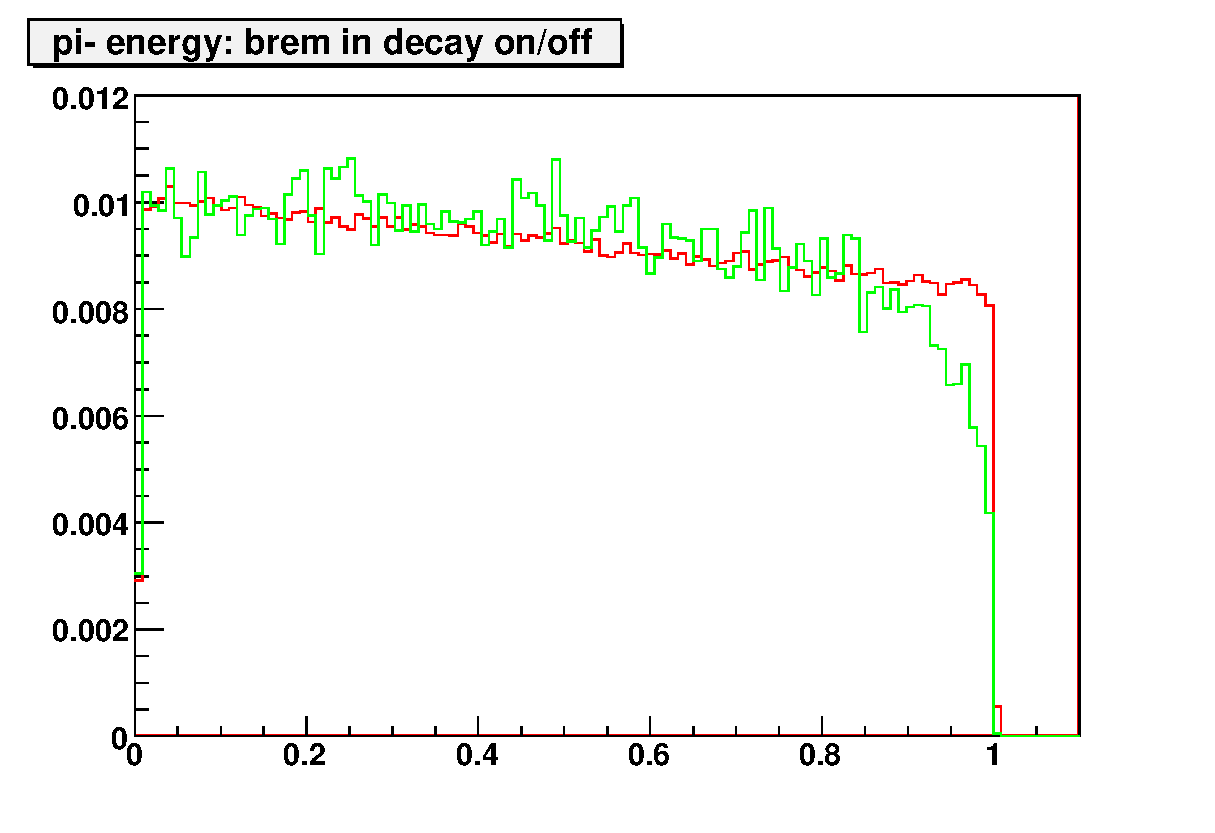
\includegraphics[scale=0.35]{bremdec.eps}
}
\subfigure[bremsstrahlung from $Z$, $\tau^+ $ and $\tau^- $ decays]{
\includegraphics[scale=0.35]{bremall.eps}
}
\caption{ Bremsstrahlung effects for longitudinal spin observables
for the cascade decay: $Z \to \tau^+ \tau^-$, $\tau^+ \to \pi^+ \nu$,  $\tau^\pm \to \pi^\pm\nu$.
$\pi^+$ energy spectrum in the Z rest-frame  is shown. The red line is for 
bremsstrahlung switched off
and green for when its effect is included. 
In the left plot, bremsstrahlung is only applied to $\tau^+ $ decay.
In the right plot, bremsstrahlung from $Z$ and  $\tau^-$ decays are
 also taken into account.
These plots has been created using a custom {\tt UserTreeAnalysis} of {\tt MC-TESTER}.
They can be recreated with the test located in the {\tt examples/testing/Ztautau} directory, see  {\tt examples/testing/README-plots} for technical details. Results are 
consistent with Fig.~5 of ref.\cite{Eberhard:1989ve}.
\label{fig:KKMC}
}
\end{figure}
\begin{figure}[h!]
\centering
\subfigure[selection C]{
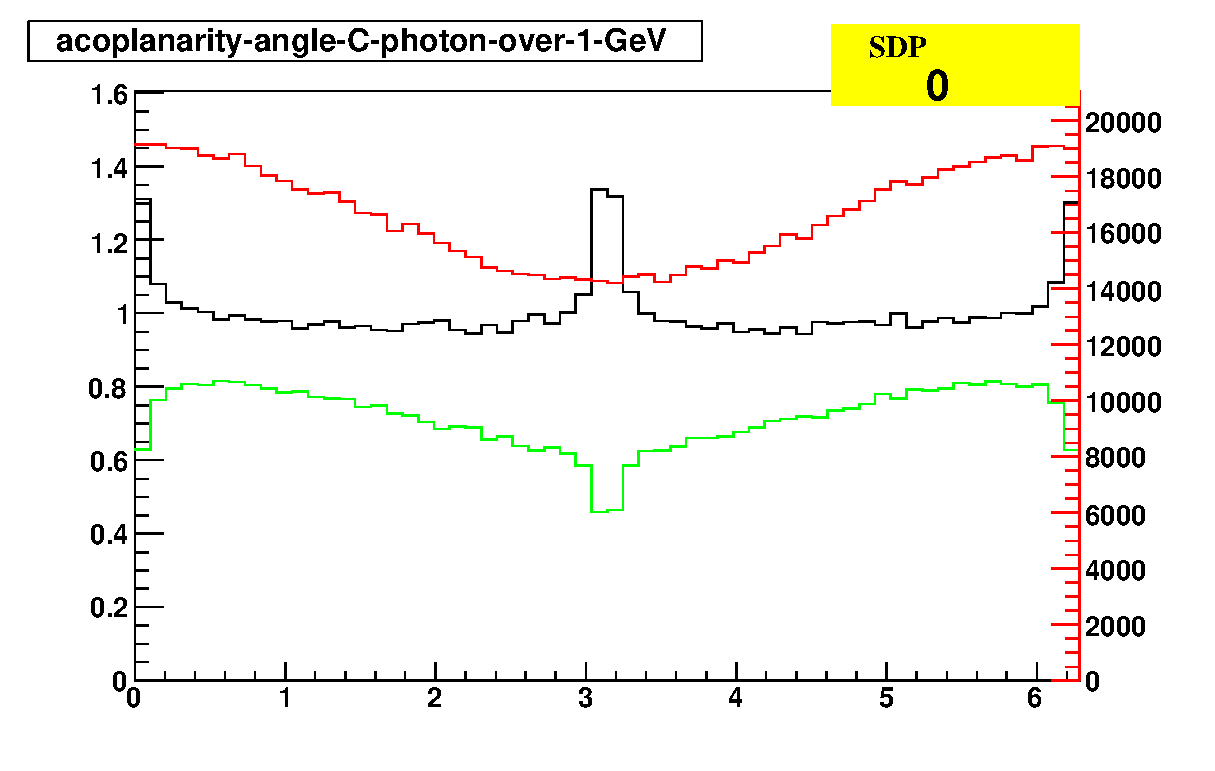
\includegraphics[scale=0.35]{coplanarity-angle-C-photon-over-1-GeV.eps}
}
\subfigure[selection D]{
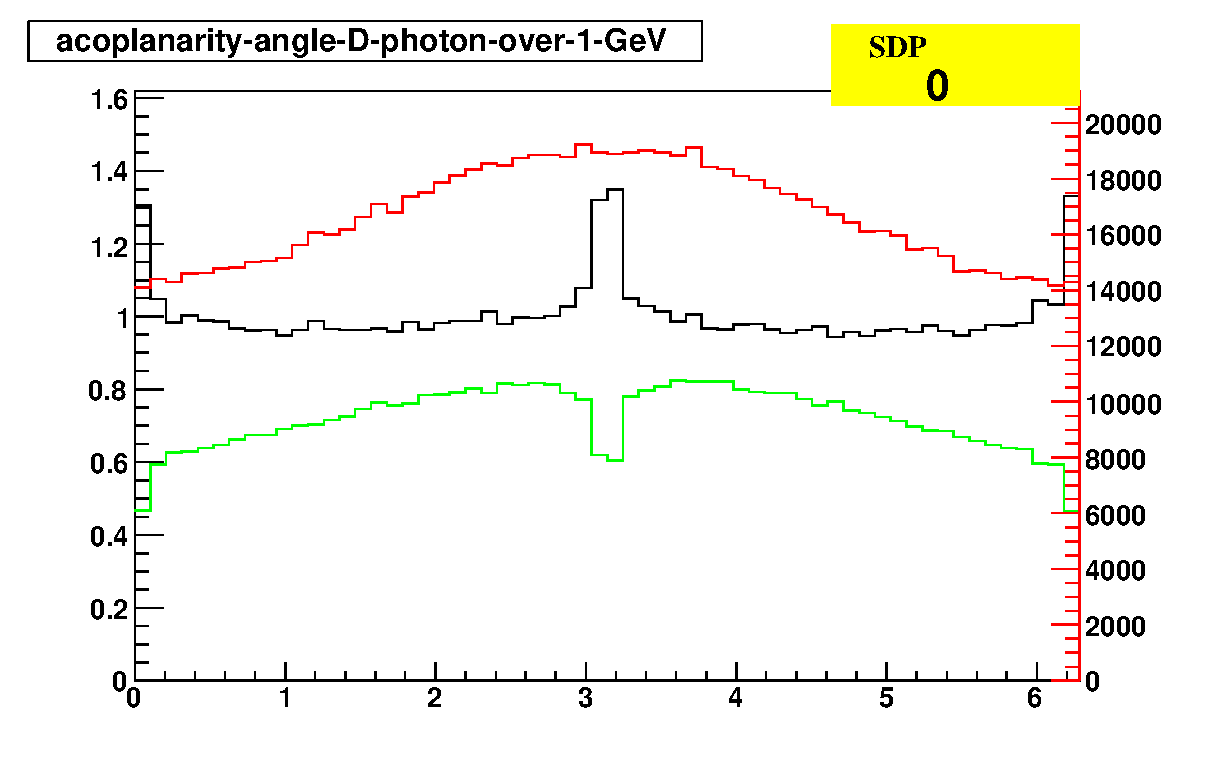
\includegraphics[scale=0.35]{coplanarity-angle-D-photon-over-1-GeV.eps}
}
\caption{Bremsstrahlung effects for transverse spin observable: In
  this plot the distribution of the acoplanarity angle between
  the $\pi^+\rho^+$ and $\pi^-\rho^-$ planes in the rest frame of the
  $\rho+ \rho^-$ pair for the scalar higgs decay chain $H\to
  \tau^+\tau^-$, $\tau^\pm \to \rho^\pm \nu_\tau$, $\rho^\pm \to
  \pi^\pm \pi^0$ is given. {\tt PHOTOS} is used to generate
  bremsstrahlung.  The red curve indicates the distribution when
  bremsstrahlung effects are ignored and the green curve shows events
  where bremsstrahlung produces photons with energy larger than 1 GeV
  in the $H$ rest frame. Note that in comparison with fig \textbf{nd-figure no.?} from
  ref~\cite{tauolaC++} the kinematical effects of hard photon emission are
  limited to a depletion/increase in the content of bins for an acoplanarity
  angle close to $0$, $\pi$ and $2\pi$. For the definition of selections C
  and D see.~\cite{Bower:2002zx}.  These plots has been created using
  a custom {\tt UserTreeAnalysis} of {\tt MC-TESTER}.  They can be
  recreated by performing the test located in the {\tt
    examples/testing/Htautau} directory, see {\tt
    examples/testing/README-plots} for technical details.
\label{fig:acoplanarity}
}
\end{figure}

In ref \cite{Adam:2008ge} a discussion of the systematic errors for the measurement of the Z cross 
section at the LHC is presented. One of the technical tests of our software is to obtain
fig 1b of that paper. In our fig \ref{fig:lineshape} we have 
reproduced that plot using {\tt PYTHIA 8.1} and {\tt PHOTOS}. Qualitatively the effect
of FSR QWD bremsstrahlung is in the two cases quite similar. A discussion
of complete electroweak corrections, as shown in fig 1a of  \cite{Adam:2008ge},
is not the purpose of our document. Let us point out however that electroweak 
non-QED corrections can be installed into the {\tt PYTHIA 8.1} - {\tt PHOTOS} simulation with 
the help of the {\tt TAUOLA} interface \cite{Davidson:2010rw}.

%nd-What do you mean by bare here? references for Horace and Winhac?
Let us present next the LHC oriented plot of Bare electron pair from $Z$
($W$) decay at the LHC with and without {\tt PHOTOS}, see fig. \ref{fig:lineshape}. It is similar to
the plots shown for Horace or Winhac.  
One should bear in mind that this is a technical test with little application directly to physics.
\begin{figure}[h!]
\centering
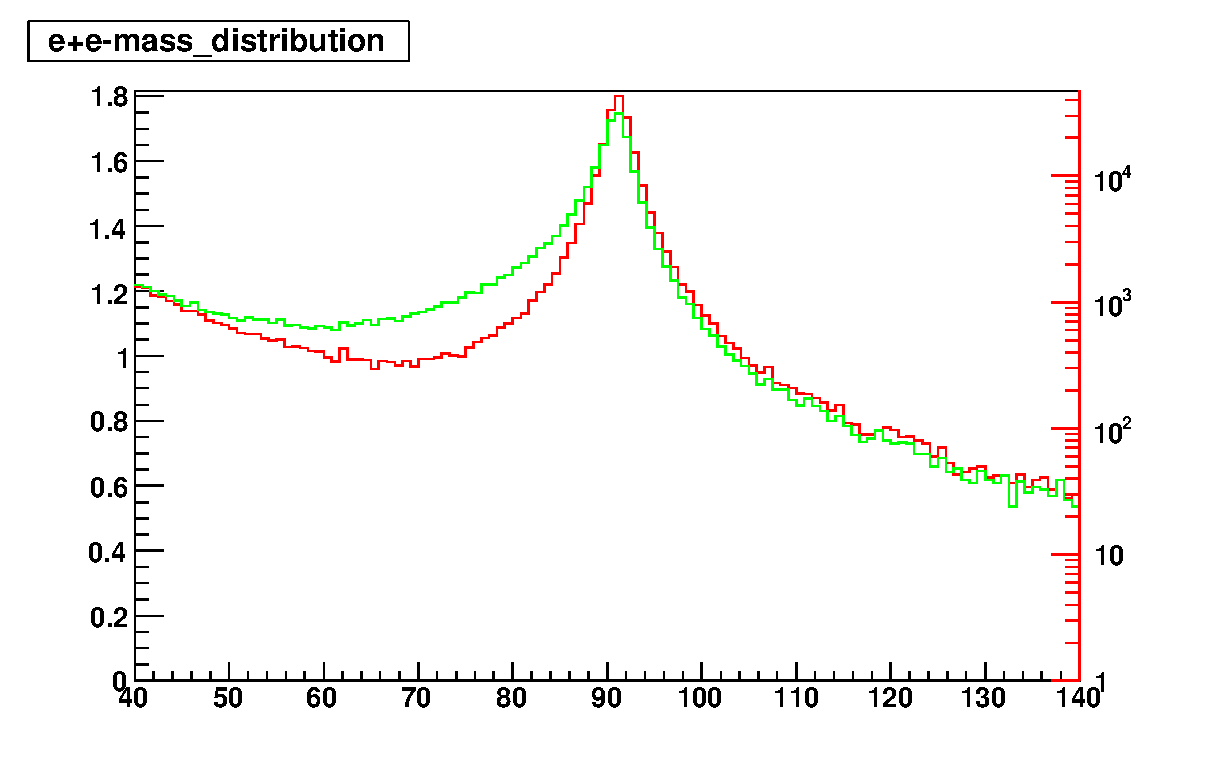
\includegraphics[scale=0.85]{lineshape.eps}
\caption{Distribution of bare $e^+e^-$ invariant mass. The green curve represents results when final state 
bremsstrahlung is generated (with the help of {\tt PHOTOS} Monte Carlo). For the red curve FSR 
bremsstrahlung is absent. The event sample is generated with the help of {\tt PYTHIA 8.1}.
The simulation of pp collisions at 14 TeV center-of-mass energy is performed.
The $Z/\gamma$ mediated hard process is used.
These plots have been created using a custom {\tt UserTreeAnalysis} of {\tt MC-TESTER}.
They can be recreated by performing the test located in the {\tt examples/testing/Zee} directory, see  {\tt examples/testing/README-plots} for technical details.
\label{fig:lineshape}
}
\end{figure}

We have also checked that {\tt PHOTOS} works for $t \bar t$ events.
For this purpose we have produced $t \bar t$ pairs in $pp$ collisions at 
14 TeV center-of-mass energy. We have produced rates for events with zero, one or
at least two photons of energy above 0.001 of the $t \bar t$ pair mass
(energies are calculated in  the hard scattering frame).
Results are given in the following table which is constructed from  
$gg \to t \bar t$ events only:

\vspace{0.3cm} 
\begin{center}
{ \begin{tabular}{c c} 
\toprule 
Final state &  Branching Ratio  $\pm$ Rough Errors \\  
\midrule
{$ \widetilde{t} t \; \;\; \;$}  &  {99.0601 $\pm$ 0.0315\%}  \\ 
%\hline 
 {$  \widetilde{t} t \gamma \;\;$} &   { 0.9340 $\pm$  0.0031\%}   \\ 
%\hline 
{$  \widetilde{t} t \gamma \gamma$}  &  { 0.0060 $\pm$  0.0002\%}  \\ 
\bottomrule
\end{tabular} 
}  
\end{center} 

%nd-what do you mean by ``rough errors'' in the table.

%nd- ``no beam was added to the list of final state particles'' maybe:
%nd- ``photons from the underlying event were ignored.'' is clearer?
10 million events were generated and a slightly modified {\tt LC-analysis} of Ref.~\cite{Golonka:2002rz}
was used for calculation of the event rates; no beam was added to the list of 
final state particles. Root files for 
differential distributions are 
collected in the directory {\tt exaples/testing/ttbar}. 

Let us now turn to an example of the test for the two photon final state configuration.
%nd-the following sentence is confusing. Do you mean KKMC with exponentiation and 2nd order matric element
% and KKMC with exponentiation and 1st order matrix element. or is the second one KKMC with 2st order matric
% element only.
We compare KKMC \cite{kkcpc:1999} with exponentiation and second order matrix element, KKMC
restricted to first order only and finally the results of {\tt PHOTOS} with exponentiation activated. As one can see from the table below, the rates for the event configurations 
where zero, one or at least two photons of energy above 1 GeV, are the same up to two
permille for the three cases and $Z\to \mu^+\mu^-$ decay. 

\begin{table}
\centering 
\begin{tabular}{lrrr} 
\toprule 
Decay channel &\multicolumn{3}{c}{ Branching Ratio $\pm$ Rough Errors   (100M event samples)} \\ 
      & {KKMC CEEX2} & {KKMC CEEX1} & {\tt PHOTOS} exp.\\ 
\midrule
 {$Z^{0} \rightarrow \mu^{+} \mu^{-} $} & {83.9190 $\pm$  0.0092\%} &{  83.7841 $\pm$  0.0092\%} & 83.8470 $\pm$ 0.0092\%\\ 
%\midrule
 {$Z^{0} \rightarrow \gamma \mu^{+} \mu^{-} $} & {14.8152 $\pm$  0.0038\%} &{  14.8792 $\pm$  0.0039\%} & 14.8589 $\pm$ 0.0039\% \\ 
%\midrule
{$Z^{0} \rightarrow \gamma \gamma \mu^{+} \mu^{-} $} & { 1.2658 $\pm$  0.0011\%} &{   1.3367 $\pm$  0.0012\%} & 1.2940 $\pm$ 0.0011\%\\ 
\bottomrule
\end{tabular}
\end{table}

Aggrement at this level is not seen in the differential distributions, see Fig.~\ref{fig:gamgam}. For example the spectrum of 
the two gamma mass is quite different between the first and second order 
exponentiation result. This is of potential interest for background simulations 
for $H \to \gamma \gamma$. In contrast, the difference between the results from {\tt PHOTOS} and CEEX2 are much smaller. {\tt PHOTOS} exploits the first order matrix element 
in a better way than exponentiation. As a consequence it reproduces terms resulting in second order leading logarithms. This observation is important not only for 
the particular case of $Z$ decay but for the general case of double bremsstrahlung in any decay as well. That is why it was worth mentioning here.
%nd-I don't know if the last sentence is needed.

\begin{figure}[h!]
\centering
\subfigure[CEEX2: red; CEEX1: green]{
\includegraphics[scale=0.35]{{M1@0001.eps}}
}
\subfigure[ CEEX2: red; PHOTOS: green]{\label{plot:b}
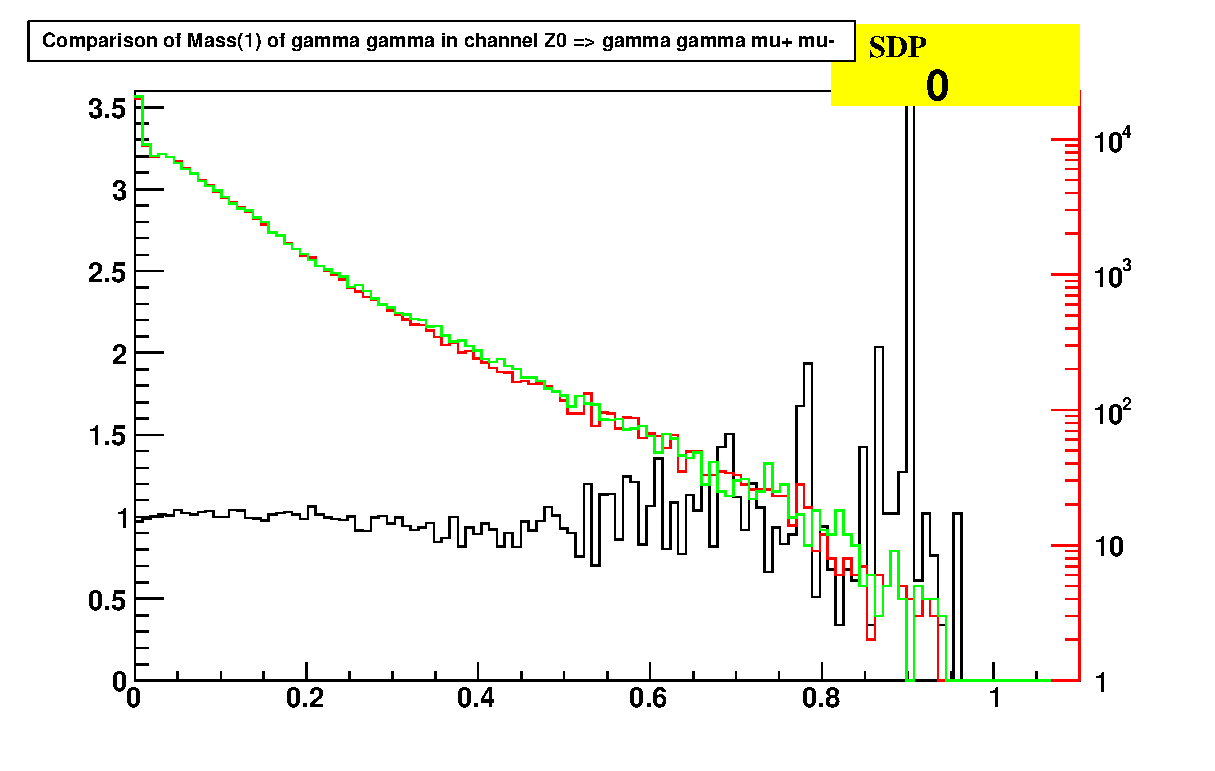
\includegraphics[scale=0.35]{b-M1@0001.eps}
}
\caption{ Spectrum of the $\gamma \gamma$ invariant mass in $Z \to \mu^+\mu^-$
decay. Events with two hard photons, both of energy above 1 GeV in the $Z$ rest 
frame are taken. Comparison are shown for CEEX2 and CEEX1 (left plot), and CEEX2 and {\tt PHOTOS}
(right plot). The prediction from {\tt PHOTOS} is clearly superior for applications aiming at
the simulation of Higgs boson backgrounds. In the case of solutions based on YFS 
exponentiation the second order matrix element must be taken into account. Plot \ref{plot:b} was obtained
from our example {\tt examples/testing/Zmumu } after adaptation of the center-of-mass energy 
(91.17 GeV) and test
energy threshold (1 GeV). Samples of 100 million events are used. 
See  {\tt examples/testing/README-plots} for technical details. Reference 
{\tt mc-tester.root} files for KKMC CEEX samples are however created outside of the distribution.
  \label{fig:gamgam}
}
\end{figure}


The numerical results collected here provide part of the program benchmarks. 
They are however of  some physics interest as well.
 Photos provides only one step in the simulation chain: 
bremsstrahlung in decays or final state bremsstrahlung. One can ask 
the question of whether such a specialized unit is of interest and whether it is not better 
to provide the complete chain as a single simulation package. Obviously this will
%nd- I would avoid saying ``complete chain'' because to experimentalists this also
%nd- includes the simulation of the detector eg. GEANT
depend on particular needs. Theoretically, final state QED corrections are 
resonably well separated from the remaining genuine electroweak corrections and 
in particular the initial state QED bremsstrahlung for quarks if for example 
Drell Yan process at the LHC is considered. 
%nd-the previous sentence is not clear. Maybe make into 2 smaller sentences.
Such separation may look like an unnecessary complication. However one should bear in mind that final state bremsstrahlung 
needs to be disentangled from detector acceptance dependencies and is not of 
interest in itself. If one wants to measure the properties of weak bosons then it 
is natural to combine their propagators defining their properties together with 
genuine electroweak corrections. 
%nd-I can't understand what you are trying to say about PHOTOS in the last two sentences.
Such a solution is now available if together 
with the PHOTOS interface of electroweak corrections as in TAUOLA Interface is 
provided. 
%nd-the previous sentence doesn't make sense (grammatically). Should
%is be something like: ``such a solution is now available if, together
%with PHOTOS, the interface of electroweak corrections as found in the
%TAUOLA Interface is provided.
Finally, sizeable initial state QED corrections are usually embodied in  units 
simulating parton showers. This may need some experimental analysis as well. 
Recently experimental data from LEP1 times are revisited \cite{Abdallah:2010tk} 
by the DELPHI collaboration. Tension between data and the theoretical description is 
mentioned. This may mean that the description of initial state QED bremsstrahlung 
at the LHC will need to be reinvestigated with the help of LHC data as well.
%nd-how does PHOTOS help with this?


\section{Summary and outlook}
We have presented a new version  of {\tt PHOTOS} Monte Carlo. The part of PHOTOS which operates on 
event records is rewritten now into C++ and takes the HepMC event record 
format for input. The physics performance of the algorithm is the same  as that of 
the {\tt FORTRAN/HEPEVT} version. Steps toward future improvements are prepared. 
Whenever algorithm for modification of an elementary decay is involved its 
kinematical configuration is boosted to the decaying particle's rest frame, with the 
$z$ axis oriented along the momentum of the first decaying particle (object) 
rest frame. 
%nd-previous sentence I would rewrite eg. ``When an elementary decay
%is modified by PHOTOS, it is tranformed to the rest frame of the
%decaying particle, with the $z$-axis orientated ...''  Also, for the
%last part is ambigious when you say ``first decaying particle''. Do
%you mean the first in the whole event, or the first in some sub-branch.
Thanks to this extension the installation of process dependent kernels
featuring the complete first order matrix element will be possible.
If of numerical interest the appropriate corrections are explained in
refs.~\cite{Golonka:2006tw,Nanava:2006vv,Nanava:2009vg}. The necessary
input is now prepared by {\tt PHOTOS}.
At present parts of the algorithm are left in {\tt FORTRAN}. This part of the code 
will be rather easy to change to C++. No obstacles are expected. However as this part of the code does not require any special data structures the expected gains,
apart from homogenity of the code, are rather minimal.  

\vskip 2 mm

\centerline{\large\bf Acknowledgements}


Useful discussions with P. Golonka during the early stage of project development and discussions 
with members of the ATLAS and CMS collaborations, and the LCG group are acknowledged.
We are especially indebted to the pilot users of the interface, in particular to:
%nd-fix
...

Partial support of Polish-French collaboration
no. 06-124 within IN2P3 through LAPP Annecy and 
during final completion of this work is
also acknowledged.

\newpage

\bibliography{Photos_interface_design}{}
\bibliographystyle{plain}






%------------------------------------------------------------------------------
\newpage
\appendix

\section{Appendix: Interface to {\tt PHOTOS FORTRAN}}
\label{Interface to PHOTOS}

This section is addressed to developers of the interface, 
and special users interested in advanced options of {\tt PHOTOS FORTRAN}.
For this purpose we describe the common blocks and routines which allow
communication between {\tt PHOTOS} and the {\tt PHOTOS} C++ Interface.

\subsection{Common Blocks}

In the following let us list the common blocks of {\tt PHOTOS} which are accessed
from C++.

\begin{description}
\item[PHOCOP] coupling constant and related parameters.
    \begin{description}
	\item[ALPHA]  \textit{double} coupling constant $\alpha_{QED}$.
	\item[XPHCUT] \textit{double} minimal energy (in units of the decaying particle mass) for photons to be explicitly generated.
    \end{description}
\end{description}

\begin{description}
\item[PHOKEY] keys and parameters controlling the algorithm options.
    \begin{description}
	\item[FSEC]   \textit{double} internal variable for algorithm options, default is FSEC-1..
	\item[FINT]   \textit{double} maximum interference weight.
	\item[EXPEPS] \textit{double} technical parameter, blocks crude level high photon multiplicity from configurations less probable than EXPEPS, default is $10^{-4}$.
	\item[INTERF] \textit{bool} key for interference, matrix element weight.
	\item[ISEC]   \textit{bool} switch for double bremsstrahlung generation.
	\item[ITRE]   \textit{bool} switch for bremsstrahlung generation up to multiplicity 4.
	\item[IEXP]   \textit{bool} switch for exponentiation mode.
	\item[IFTOP]  \textit{bool} switch for photon emission in top pair production in quark (gluon) pair annihilation.
    \end{description}
\end{description}

\begin{description}
\item[PHSEED] common block for a copy of the Marsaglia and Zaman random number generator used in the {\tt FORTRAN} part of {\tt PHOTOS}.
    \begin{description}
	\item[ISEED[ 2]]  \textit{int} seed values, default is  ISEED[ 1]=1802, ISEED[ 2]=9373
	\item[I97]        \textit{int} internal variable of the random number generator.
	\item[J97]        \textit{int} internal variable of the random number generator.
	\item[URAN[ 97]]  \textit{double} internal variable of the random number generator.
	\item[CRAN]       \textit{double} internal variable of the random number generator.
	\item[CDRAN]      \textit{double} internal variable of the random number generator.
	\item[CMRAN]      \textit{double} internal variable of the random number generator.
    \end{description}
\end{description}

\begin{description}
\item[PHLUPY] debug messages handling.
    \begin{description}
    \item[IPOIN]  \textit{int} messages above this value will not be displayed.
	\item[IPOINM] \textit{int} messages below this value will not be displayed.
    \end{description}
\end{description}

\begin{description}
\item[PH\_PHOQED] supplement for PH\_HEPEVT event record to block emission 
from some particles.
    \begin{description}
    \item[QEDRAD[ 10000]]  \textit{bool} flag enabling {\tt FORTRAN} users
    to block emission from particles stored in PH\_HEPEVT. Not used in 
     our interface.
    \end{description}
\end{description}

\subsection{Routines}

In the following let us list routines which are called from the interface.

\begin{description}
\item[PHOINI] initialize the generator, use as input the content of common blocks. \\
  Return type: \textit{void} \\
  Parameters: none
\end{description}

\begin{description}
\item[PHODMP] prints out the content of HEPEVT. \\
  Return type: \textit{void} \\
  Parameters: none
\end{description}

\begin{description}
\item[PHOTOS\_MAKE] {\tt FORTRAN} part of interface. \\
  Return type: \textit{void} \\
  Parameters:
  \begin{enumerate}
    \item \textit {int id} ID of particle from which {\tt PHOTOS} starts processing. In the C++ case the importance of this parameter is limited as only one branch is in HEPEVT at a time.
  \end{enumerate}
\end{description}

\begin{description}
\item[PHCORK] initializes kinematic corrections. \\
  Return type: \textit{void} \\
  Parameters:
  \begin{enumerate}
    \item \textit {int modcor} type of correction. See {\tt FORTRAN} documentation for details.
  \end{enumerate}
\end{description}

\section{Appendix: User Guide}
\label{sec:User Guide}

\subsection{Installation}
\label{sec:Installation}
The main interface library requires that {\tt HepMC} \cite{Dobbs:2001ck} (version 2.04 or later)  has been installed
and its location has been provided during the configuration step. This is sufficient to compile the interface and to run the simple, standalone example.

However, in order to run more advanced examples located in the {\tt /examples} directory, it is required to install also:

\begin{itemize}
  \item {\tt ROOT} \cite{root-install-www} version 5.18 or later
  \item {\tt PYTHIA 8.1} \cite{Sjostrand:2007gs} or later. {\tt PYTHIA 8.1} must be compiled with {\tt HepMC} 2.xx
        so that the {\tt PYTHIA} library {\tt hepmcinterface} exists.
  \item {\tt MC-TESTER} \cite{Golonka:2002rz,Davidson:2008ma} version 1.24 or later.
        Do not forget to type {\tt make libHepMCEvent} after compilation of {\tt MC-TESTER} is done.
  \item {\tt TAUOLA} \cite{Davidson:2010rw} version 1.02 or later.
\end{itemize}

In order to compile the {\tt PHOTOS} C++ Interface:
\begin{itemize}
 \item Execute {\tt ./configure} with the additional command line options:
   \subitem {\tt --with-HepMC=$<$path$>$} provides the path to the {\tt HepMC} installation directory. One can also set the {\tt HEPMCLOCATION} variable instead of using this directive. This path is required for the interface to compile.
   \subitem {\tt --prefix=$<$path$>$} provides the installation path. The {\tt include} and {\tt lib} directories will be copied there if {\tt make install} is executed later. If none has been provided, the default directory for installation is {\tt /usr/local}.
 \item Execute {\tt make}
 \item Optionally, execute {\tt make install} to copy files to the directory provided during configuration.
\end{itemize}

The {\tt PHOTOS} C++ interface will be compiled and the {\tt /lib} and {\tt /include} directories will contain the appropriate libraries and include files.

In order to compile the examples, compile the {\tt PHOTOS} C++ interface and enter the {\tt /examples} directory and:
\begin{itemize}
  \item Execute {\tt ./configure} to determine which examples can be compiled.
        Additional paths can be provided as command line options:
   \subitem {\tt --with-Pythia8=$<$path$>$} provides the path to the {\tt Pythia8} installation
            directory. One can set the {\tt PYTHIALOCATION} variable instead of using this directive.
            This path is required for all examples and tests.
   \subitem {\tt --with-MC-Tester=$<$path$>$} provides the path to the {\tt MC-TESTER} installation
            directory (the {\tt libHepMCEvent} must be compiled as well, see \cite{Davidson:2008ma}
			for more details). One can set the {\tt MCTESTERLOCATION} variable instead of using this
			directive. This path is required for all additional examples and tests.  This option
			implies that {\tt ROOT} has already been installed (since it is required by {\tt MC-TESTER}).
			The {\tt ROOT} directory {\tt bin} should be listed in the variable {\tt PATH} and the {\tt ROOT}
			libraries in {\tt LD\_LIBRARY\_PATH}.
   \subitem {\tt --with-Tauola=$<$path$>$} provides the path to the {\tt TAUOLA} installation directory.
            One can set the {\tt TAUOLALOCATION} variable instead of using this directive.
			This path is required for additional examples only.
  \item execute {\tt make}
\end{itemize}

If neither {\tt Pythia8} nor {\tt MC-TESTER} are present, only the simple example will be provided. The {\tt /examples} directory will contain the compiled example files.

\subsection{Elementary Tests}
\label{sect:elem}

%nd-maybe the commands to execute the stand-alone test should be meantioned here.
%nd-So that the user knows how to conduct the elementary tests after they install PHOTOS.
The most basic test which should be performed is verification that the interface is installed correctly, that all
photons are indeed added by the program and that energy momentum conservation is preserved.

Once correct execution of the basic program steps have been confirmed,
step one of the program installation tests  is completed\footnote{
We have  performed such  tests for all choices of the {\tt HepMC} event record obtained 
from  {\tt PYTHIA 8.1} processes and 
listed later in the paper. Further  options for initializations 
(parton shower hadronization or QED bremsstrahlung on/off etc.) were studied.
This installation step  was a necessary one of program development as well.}.

In principle, these tests have to be performed for any new hard 
process and after any new installation. This is to ensure that 
information is passed from the event record to the interface 
correctly and that physics information is filled into {\tt HepMC} 
in the expected manner. Misinterpretation of the event record content may result in 
faulty generation by {\tt PHOTOS}.


\subsection{Executing Examples}

Once elementary tests are completed one can turn to the more advanced ones.
The purpose is not only to validate the installation but to demonstrate how the
interface can be used.

The examples can be run by executing the appropriate {\tt .exe} file in the {\tt /examples} directory.
In order to run some more specific tests for the following processes:
$H \rightarrow \tau^+ \tau^-$, $ e^+ e^- \rightarrow t \bar t$,
$W \rightarrow e \nu_e$, $W \rightarrow \mu \nu_\mu$,
$Z \rightarrow e^+ e^-$, $Z \rightarrow \mu \mu$ or $Z \rightarrow \tau^+ \tau^-$,
the main programs residing in subdirectories of {\tt /examples/testing} should be executed.
In all cases the following actions have to be performed:

\begin{itemize}
  \item Compile the {\tt PHOTOS } C++ Interface as well as the examples. 
 \item  Check that the appropriate system variables are set: normally set by the script \\
{\tt /configure.paths.sh} (the configuration step mentions this script).
  \item Enter the {\tt /examples/testing} directory. Modify test.inc if needed.
  \item Enter the chosen directory and execute {\tt make}.
\end{itemize}

The appropriate .root files as well as .pdf files generated by {\tt MC-TESTER}
will be created inside the chosen directory. One can execute 'make clobber' to
clean the directory. One can also execute 'make' inside the {\tt /examples/testing}
directory to run all available tests one after another. New source
code changes can easily be validated in this way.
Most of the tests are run using {\tt examples/photos\_pythia\_example.exe};
only $H \rightarrow \tau^+ \tau^-$ and $Z \rightarrow \tau^+ \tau^-$ require
{\tt examples/tauola\_photos\_pythia\_example.exe} to be compiled as well.
After generation booklets will be produced with comparisons to the benchmark files.
Note that $W \rightarrow e \nu_e$, $W \rightarrow \mu \nu_\mu$ and $Z \rightarrow \mu \mu$
examples  show differences higher than statistical error. This is because  photon symmetrization
was used in the benchmark files generated with {\tt KKMC}, and not in the one generated with {\tt PHOTOS}.
In the case of {\tt KKMC} the generated photons are strictly ordered in energy. In the case of {\tt PHOTOS}
they are not. Nonetheless, on average the second photon has a smaller energy than the one written as the first
in the event record.


A set of benchmark {\tt MC-TESTER} root files are packed with the interface
distribution in the subdirectories of {\tt examples/testing/}. They can be used
as examples to start new work or simply to construct comparison
plots to validate new versions or new installations of the {\tt PHOTOS} interface.

In Appendix \ref{sec:User Configuration} possible modifications to the  
example's settings are discussed. This may be interesting as an initial step for user's 
physics studies.  The numerical results of some of these tests are collected in Section \ref{sec:results}
and can be thus reproduced by the user.

\subsection{How to run {\tt PHOTOS} with other generators}
If a user is building a large simulation system they may want to avoid our 
infrastructure and load only the libraries. For that purpose our stand-alone 
example is a good starting point.

In order to link the libraries to the user's project, both the static libraries and shared objects are
constructed. To use the {\tt PHOTOS} interface in an external project, additional 
compilation directives are required. For the static libraries:
\begin{itemize}
  \item add {\tt -I<PhotosLocation>/include } at the compilation step,
  \item add {\tt <PhotosLocation>/lib/libPhotosCxxInterface.a } and\\
        {\tt <PhotosLocation>/lib/libPhotosFortran.a } at the linking step.
\end{itemize}
For the shared objects:
\begin{itemize}
  \item add {\tt -I<PhotosLocation>/include } at the compilation step,
  \item add {\tt -L<PhotosLocation>/lib } along with {\tt -lPhotosCxxInterface } at the linking step.
  \item  {\tt PHOTOS} libraries must be provided for the executable; eg. with the help of {\tt LD\_LIBRARY\_PATH}.
\end{itemize}
%nd-how do you link the fortran libraries in the case of shared objects?
{\tt <PhotosLocation>} denotes the path to the {\tt PHOTOS} installation directory.
In most cases it should be enough to include {\tt Photos.h} and {\tt PhotosEvent.h}
within a user's program and use the {\tt PHOTOS} class for configuration and {\tt PhotosEvent}
for event processing.

\section{Appendix: User Configuration}
\label{sec:User Configuration}

\subsection{Suppress Bremsstrahlung}
\label{section:suppress}

In general, {\tt PHOTOS} will attempt to generate bremsstrahlung for every 
branching point in the event record. This is of course not always appropriate.
Already inside {\tt FORTRAN}, bremsstrahlung is not generated for vertices involving gluons or quarks 
(with the exception of top quarks). 
%nd- Clarify FORTRAN. Do you mean in the FORTRAN part of the new PHOTOS. Or the old FORTRAN Interface to PHOTOS?

This alone is insufficient. By default we suppress bremsstrahlung
generation for vertices like $l^\pm \to l^\pm \gamma$ because a
``self-decay'' is unphysical. We can not request that all incoming
and/or outgoing lines are on mass shell, because it is not the case in
cascade decays featuring intermediate states of sizeable width. If a
parton shower features a vertex with $l^\pm \to l^\pm \gamma$ with the
virtuality of the incoming $l^\pm$ matching the invariant mass of the
outgoing pair then the action of {\tt PHOTOS} at this vertex will
introduce an error.  This is prevented by forbidding bremsstrahlung
generation at vertices where one of the decay products has a flavour
which matches the flavour of an incoming particle.


Some exceptions to the default behaviour may be necessary. For example
in cascade decays, the vertex $\rho \to \rho \pi$ may require the
PHOTOS algorithm to be activated.
%nd-for my own interest: What is special about rho -> rho pi? isn't this unphysical as well?
Methods to reenable these previously prevented cases, or to prevent generation in special
branches have been introduced and are presented in the next section.
This may be necessary for the combination of consecutive branches. For
example if bremsstrahlung in leptonic $\tau$ decay is generated by
programs prior to {\tt PHOTOS}, and the decay is constructed in HepMC as the cascade
$\tau^\pm \to W^\pm \nu$, $W^\pm \to l^\pm \nu$, {\tt PHOTOS} must
be prevented to act on both verticies. One
can also think of the following type of special case: if a vertex $q
\bar q \to l^\pm l^\mp$ is found then it should not be ignored but
passed for generation as $q \bar q \to Z \to l^\pm l^\mp$ where
the intermediate Z is created internally for {\tt PHOTOS}. \\ \\ 
%nd-From the last statement about qq->Z->ll, it's not clear to me whether PHOTOS does this by default,
%doesn't do it by default but has options for doing it, or whether it's something the user
%has to do in themselves.

For user's convenience the following configuration methods are provided:
\begin{itemize}
 \item {\tt Photos::suppressBremForDecay(daughterCount, motherID, d1ID, d2ID, ...)} \hfill \\
       The basic method of channel suppression. The number of daughters,
	   PDGID of the mother and the list of PDGIDs of daughters must be provided.
	   There's no upper limit to the number of daughters.
	   If a decay with the matching pattern is found, {\tt PHOTOS} will skip the decay.
 \item {\tt Photos::suppressBrem(0, motherID)} \hfill \\
       When only the PDGID of the mother is provided, {\tt PHOTOS} will skip all decay channels
	   of this particle. Note, that the number of daughters must still be provided,
	   which in this case is zero.
 \item {\tt Photos::suppressBremForBranch(daughterCount, motherID, d1ID, d2ID, ...)} \hfill \\
       {\tt Photos::suppressBremForBranch(0, motherID)} \hfill \\
       The usage of these methods is similar to the above function. The difference is
	   that {\tt PHOTOS} will skip not only the corresponding channel,
	   but also all consecutive decays of its daughters, making {\tt PHOTOS} skip the entire branch
	   of decays instead of just one listed decay.
 \item {\tt Photos::suppressAll() }
       All branchings will be suppressed except those that are forced using the methods
	   described in the next section.
 \item \textbf{Example:} \hfill \\
{\tt Photos::suppressBremForDecay(4, 15, 16, -211, 300, -400); } \\
{\tt Photos::suppressBremForDecay(2, -15, -16, 211); } \\
{\tt Photos::suppressBremForDecay(0, 211); } \\
\emph{If the decays {\tt 15 => 16, -211, 300, -400} or {\tt -15 => -16, 211} are found, they will be skipped by {\tt PHOTOS}. In addition, all decays of particle {\tt 211} will also be skipped. Note, that the minimum number of parameters that must be provided is two - the number of daughters (which can be zero) and the mother PDGID.} \\ \\
{\tt Photos::suppressBremForBranch(2, 15, 16, -211); } \\
\emph{When a decay {\tt 15 => 16, -211 } is found, it will be skipped by {\tt PHOTOS} along with the decays of particle 16, -211 and all their daughters. In the end, the whole decay tree starting with {\tt 15 => 16, -211} will be skipped.}
\end{itemize}
%nd-might be nice to use the particle symbols above instead of the PDGID. 
%eg. ``15 => 16 ...'' to ``%\tau^- \rightarrow \nu_{\tau} ...$

\subsection{Force {\tt PHOTOS} processing }
\label{section:force}

Forcing PHOTOS to process a branch can be used in combination with
suppressing all branches i.e. to allow selection of only particular
procesess for bremstrahlung generator.

Forcing processing using the methods below has higher priority than the suppressing described
in the previous section, therefore even if both forcing and suppressing of the same
branch or decay is done (regardless of order), the processing will not be
suppressed.

\begin{itemize}

 \item {\tt Photos::forceBremForDecay(daughterCount, motherID, d1ID, d2ID, ...)} \hfill \\
       {\tt Photos::forceBremForDecay(0, motherID)} \hfill \\
       The usage of this routine is similar to {\tt Photos::suppressBremForDecay(...)}
	   described in the previous section. If a decay with the matching pattern is found,
	   {\tt PHOTOS} will be forced to process the corresponding decay, even if it was suppressed
	   by any of the methods mentioned in the previous section.
 \item {\tt Photos::forceBremForBranch(daughterCount, motherID, d1ID, d2ID, ...)} \hfill \\
       {\tt Photos::forceBremForBranch(0, motherID)} \hfill \\
       The usage is similar to the above function. The difference is
	   that {\tt PHOTOS} will force, not only the corresponding channel,
	   but also all consecutive decays of its daughters, making {\tt PHOTOS} process the entire branch
	   of decays instead of just one listed decay.
 \item \textbf{Example:} \hfill \\
{\tt Photos::suppressAll(); } \\
{\tt Photos::forceBremForDecay(4, 15, 16, -211, 300, -400); } \\
{\tt Photos::forceBremForDecay(2, -15, -16, 211); } \\
{\tt Photos::forceBremForBranch(0, 211); } \\
\emph{Since suppression of all processess is used, only the listed decays will be processed, these are
{\tt 15 => 16, -211, 300, -400}, {\tt -15 => -16, 211} and all instances of the decay of {\tt 211} and
its descendants.}
\end{itemize}

\subsection{Use of the {\tt processParticle} and {\tt processBranch} methods}
\label{PHOTOSgun}

In Section~\ref{sect:Outline} the algorithm for processing a whole
event record is explained and is provided through the {\tt process()}
method.  To process a single branch in the event record, in a way
independent of the entire event, another simple method is provided.

\begin{itemize}
  \item {\tt Photos::processParticle(PhotosParticle *p) } \hfill \\
		The main method for processing a single particle. A pointer to a particle must
		be provided. From this particle a branch containing its mothers and daughters
		will be created and processed by {\tt PHOTOS}.
  \item {\tt Photos::processBranch(PhotosParticle *p) } \hfill \\
 		When a pointer to particle is provided, {\tt PHOTOS} will process the whole decay
		branch starting from the particle provided.
\end{itemize}

An example, {\tt single\_photos\_gun\_example.c}, is provided in the directory {\tt /examples}
showing how this functionality can be used to process the decay of selected particles.
$Z0 \rightarrow \tau^+ \tau^-$ decays are generated and the event record is traversed
searching for the first $\tau^-$ particle in the event record.
Instead of processing the whole event, only the decay of $\tau^-$ is processed by {\tt PHOTOS}.


\subsection{Logging and Debugging}
\label{App:Logging}
This section describes the basic functionality of the logging and debugging tool.
For details on its content we address the reader to comments in the {\tt /src/utilities/Log.h} header file.

Let us present however some general scheme of the tool's
functionality.  The {\tt PHOTOS} interface allows control over the
amount of message data displayed during program execution and
provides a basic tool for memory leak tracking. The following
functions can be used from within the user program after including the
{\tt Log.h} file:
\begin{itemize}
  \item {\tt Log::Summary() } - Displays a summary of all messages.
  \item {\tt Log::SummaryAtExit() } - Displays the summary at the end of a program run.
  \item {\tt Log::LogInfo(bool flag) } \\
        {\tt Log::LogWarning(bool flag) } \\
        {\tt Log::LogError(bool flag) } \\
        {\tt Log::LogDebug(int s, int e) } \\
        {\tt Log::LogAll(bool flag)} \\
        Turns the logging of \textit{info}, \textit{warning}, \textit{error} and \textit{debug} messages on or off depending
        on the flag value being true or false respectivly. In the case of \textit{debug} messages - the range of message codes
        to be displayed must be provided. By default, only \textit{debug} messages
        (from 0 to 65535) are turned off. If the range is negative ($s>e$) \textit{debug} messages
        won't be displayed. The last method turns displaying all of the above messages on and off.
  \item {\tt Log::LogPhlupa(int from, int to) } \\
        Turns logging of debug messages from the {\tt FORTRAN} part of the program on and off.
\end{itemize}
%nd-what do the debug codes 0-65535 mean? Is there somewhere that the user can find a list of all the possible
%messages?

Additionally, the option {\tt Log::SetWarningLimit(int limit)} is available, allowing
only the first {\tt `limit'} warnings to be displayed. The default for {\tt limit} is 100. 
If {\tt limit}=0 is set then there are no limits on the number of warnings to be display.

The memory leak tracking function allows checking of whether all memory allocated within {\tt PHOTOS Interface}
 is properly released. However, using the debug option significantly increases the amount of time needed for 
each run. Its  use is therefore recommended  for debugging purposes only. In order to use this option
 modify {\tt make.inc} in the main directory by adding the line: \\
\\ {\tt DEBUG = -D"\_LOG\_DEBUG\_MODE\_" } \\ \\
Recompile the interface.
Now, whenever the program is executed a table will be printed at the end of the run,
listing all the pointers that were not freed, along with the memory they consumed.
If the interface works correctly without any memory leaks, one should get an empty table.

It is possible to utilise this tool within the user program, however there are a few limitations.
The debugging macro from "Log.h" can create compilation errors if one compiles
it along with software which has its own memory management system (e.g. {\tt ROOT}).
To make the macro work within a user's program, ensure that {\tt Log.h} is the last header file
included in the main program.
It is enough to  compile the program with the {\tt -D"\_LOG\_DEBUG\_MODE\_" } directive added,
or {\tt \#define \_LOG\_DEBUG\_MODE\_ } placed within the program before inclusion of
of the {\tt Log.h} file
\footnote{Note that {\tt Log.h } does not need to be included within
the user program  for the memory leak tracking tool to be used only for the {\tt PHOTOS} interface.
}.

\subsection{Other User Configuration Methods}
\label{subsection:other_methods}

%nd-I might have missed it, but shouldn't there also be a section on how to config.
%photos for physics. eg. stuff like turning exponentiation on/off etc. Most of the
%stuff in the common blocks PHOCOP and PHOKEY should be settable through C++ as well
%shouldn't it?

The following auxiliary methods are prepared. They are useful for initialization 
or are introduced for backward compatibility.

\begin{itemize}
  \item {\tt Photos::setSeed(int iseed1, int iseed2)} \\
        Set the internal {\tt FORTRAN} RANMAR random generation seed values.
   \item {\tt Photos::maxWtInterference(double interference)} \\
        Set the maximum interference weight. The default is 2.
\end{itemize}

\subsection{Creating advanced plots and custom analysis}
\label{App:Plots}

%nd-I would be inclined to move this section to after B.3 Executing Examples.

In Section \ref{sec:results}, we've presented results of a non-standard
analysis performed by {\tt MC-Tester}. Figure \ref{fig:lineshape} has been
obtained using a custom {\tt UserTreeAnalysis} located in the file {\tt ZeeAnalysis.C}
residing in the {\tt examples/testing/Zee} directory. This file serves as an
example of how custom analysis can be performed and how new plots can be
added to the project with the help of {\tt MC-Tester}.

The basic {\tt MC-Tester} analysis contains methods used by pre-set examples
in the {\tt examples/testing} directory to limit the number of soft photons generated
by {\tt PHOTOS}. Its description and usage have already been documented in \cite{Davidson:2008ma}.
The content of {\tt ZeeAnalysis.C} is identical to the default {\tt UserTreeAnalysis}
of {\tt MC-Tester} with the only addition being a simple method to create
the previously mentioned plot.

In order to create the $t \bar t$ example that {\tt PHOTOS} is able to process,
two additional routines had to be added to {\tt photos\_pythia\_example.c}.
These routines - {\tt electronToGluon} and {\tt fixForMctester} are necessary
due to the uniqueness of the generated process.
%nd-I don't know much about the t tbar example. Is the electronToGluon method a fix
%for the event record so that PHOTOS works on it correctly, or it is just a fix for MC-TESTER?
%If the extra method is always necessary for PHOTOS to work correctly on ttbar events maybe it should
%be highlighted more. eg. meantioned in the results section for the ttbar example.

Since {\tt MC-Tester} is not designed to analyze processes involving
multiple incoming particles, we've used a simple method similar to that previously
used in the {\tt FORTRAN} examples {\tt LC\_Analysis} mentioned in \cite{Golonka:2002rz}, Section 6.1. However,
this method proved to be hard to implement with the current version of the {\tt HepMC}
interface of {\tt MC-Tester}, therefore a special routine had to be added
to add similar modifications to the {\tt HepMC} event. 
%nd-I would remove the previous sentence.
This modification transforms the $X Y \rightarrow t \bar t$ process to
the $100 \rightarrow Y t \bar t$ process, where the momentum of the
special particle $100$ is $X + 2*Y$ so that momentum remains conserved
within the vertex. With this modification, {\tt MC-Tester} can be set
up to analyze the particle $100$ in order to get a desirable results.

%------------------------------------------------------------------------------
\newpage

%nd-the task list should be removed at some point.
\section*{Task List}
In this section we provide a check-list of incomplete tasks.
This could be used as a guide for project planning and is foreseen
to be a working document. 

(prioritized: {\bf 1} - Highest priority. The program should not be
released without this task being completed. {\bf 2} - Medium priority.
It should be clearly documented for developers and users that this task has not
been completed. {\bf 3} - Lowest priority such as a long term goal 
for the project).

\subsection*{Functionality}
\begin{itemize}
  \item[\ding{111}]{\bf 1} - Complete example t tbar
  \item[\ding{111}]{\bf 2} - Remove dead {\tt FORTRAN} code
  \item[\ding{111}]{\bf 2} - Rewrite parts on HEPEVT type data structure
  \item[\ding{111}]{\bf 3} - Move {\tt FORTRAN} remnants to C++
\end{itemize}

\subsection*{Testing}
\begin{itemize}
  \item[\ding{111}]{\bf 1} - Long run root files for tests e+e- and pp
  \item[\ding{111}]{\bf 1} - missing plots for documentation benchmarks
  \item[\ding{111}]{\bf 2} - event record options
  \item[\ding{111}]{\bf 3} - further plots of some interest
\end{itemize}

\subsection*{Usability}
\begin{itemize}
  \item[\ding{111}]{\bf 1} - paper complete
  \item[\ding{111}]{\bf 1} - READMES 
  \item[\ding{111}]{\bf 2} - paper cleaning
  \item[\ding{111}]{\bf 2} - User interaction and resulting fixes
  \item[\ding{111}]{\bf 3} - Doxygen documentation update
\end{itemize}


\end{document}
